\documentclass{nime-alternate}

\begin{document}
%
% --- Author Metadata here ---
\conferenceinfo{NIME'11,}{30 May--1 June 2011, Oslo, Norway.}

\title{BeepinBalls - Handheld Spherical\linebreak Synthesizers for Sonifying Play}

\numberofauthors{2}
\author{
% 1st. author
\alignauthor
Michael Rotondo\\
       \affaddr{CCRMA, Department of Music}\\
       \affaddr{Stanford University}\\
       \affaddr{Stanford, California, USA}\\
       \email{mrotondog@ccrma.stanford.edu}
% 2nd. author
\alignauthor
Francesco Georg\\
       \affaddr{CCRMA, Department of Music}\\
       \affaddr{Stanford University}\\
       \affaddr{Stanford, California, USA}\\
       \email{fgeorg@stanford.edu}
}
\maketitle
\begin{abstract}
We created three miniature self-contained synthesizers which are enclosed in small toy balls and sonify the act of playing with the balls. We specifically focused on designing the synthesis to enhance the experience of juggling, due to its varied and expressive composition of motions such as throws, catches, and carries of multiple balls. 

The synthesizer consists of an Arduino microcontroller, accelerometer, synthesis chip and circuitry, and a 9-volt battery and speaker, all of which fit inside a standard 9'' circumference ``wiffle''-style ball. The Arduino runs custom firmware designed to sample the accelerometer as accurately as possible while maintaining an internal state machine that attempts to intelligently model any forces currently being applied to the ball. The properties of this state machine are then translated through a sound design ``layer'' into commands for the synthesizer chip.

The circuitry and construction of the  balls were designed to be easily reproducible, as part of our intention with this project was to create a new experience that anyone could enjoy, as opposed to creating a unique or singular object.
\end{abstract}

\keywords{Sonification, accelerometer, Soundgin, juggling, Arduino, hand-held}

\section{Introduction}

Throwing and catching a ball is one of the oldest and most fundamental forms
of play that humans engage in. As our societies developed, we extended 
this simple play experience into complex sports and games, and jugglers 
have taken the basic form to extremes, with 
some able to keep 10 balls in the air at once. At the most simple level,
however, throwing and catching a ball is still an effective way for young 
children to increase their motor skills, learn firsthand about the physics of
force and materials, and to build social awareness by playing catch with other
kids.

Our goal with BeepinBalls was to add a sonic dimension to this existing play
experience. We designed and created a ball that contains all the necessary
circuitry and equipment to synthesize and output sound corresponding to
the motion of the ball itself. We focused our design in particular on 
improving the experience of juggling, but it is generally an improvement
in all types of play. We think it improves the experience of playing with a ball
in three ways.

The simplest way in which sound changes ball play is by adding new sensory rewards.
We play with balls at the youngest age simply for the pleasurable sensations:
the sight of the ball arcing through the air or bouncing off the ground, the
tactile feeling of releasing and catching the ball, and possibly the sound of the
ball hitting our hand as we catch it. Adding pleasing and variable sound
synthesis which correlates with the other senses (e.g. pitch corresponds to height,
vibrato corresponds to spin etc) increases the extent to which exploratory
play is rewarded with new positive outcomes, which is basically the
definition of ``fun''. This is also the method by which young children self-educate
about physical laws, so enriching the experience serves to add new opportunities
for learning.

This additional feedback channel also serves to increase the ``learnability''
of complex tasks such as juggling. With additional input about our own
performance, we should be able to learn more quickly how to develop our
skills to achieve the desired outcome. In this case, the combination of the
rhythmic nature of juggling and the accentuation of catches by the synthesizer
inside the BeepinBalls lets us hear much more accutely when our juggling is
``off-tempo'', as humans are well attuned to hearing imperfect rhythms.

Lastly, but related to the previous two enhancements, the additional output 
dimension and its intuitive controllabilty by the user makes the experience
of play much more expressive. By varying throws, catches and carries in ways
that otherwise might not have been observably different, the player's intent 
can be manifested through the synthesized sound of the BeepinBalls.

Because each of these enhancements scale near-linearly with each additional
BeepinBall, we decided to make three of them. This also allowed us to test 
their feasability as juggling balls, and to tune the hardware and circuit design
to be easier to reproduce.

\section{Design and Construction}

Each BeepinBall consists of a 9''-circumference ``wiffleball'' which has been
sawed in half and reassembled around the circuitry, speaker and battery. The
enclosure was chosen for its size, cheapness, durability, and perforated shell.
These qualities mean that the BeepinBalls are able to withstand shock, and are 
easy to hold, throw and catch. They also mean that we can assemble them
while still having access to the power switch and mini-USB port on the Arduino,
and that the speaker is not muffled or muted.

Inside the ball is a perfboard which contains an Arduino Nano v3.0, based on
the ATmega 328 microcontroller, along with a 3-axis accelerometer breakout board
and a 7805 5-volt power regulator. On another perfboard is a Soundgin synthesizer,
along with a 10Mhz crystal to clock it, a simple RC filtering circuit and an
LM386 audio power amplifier. The Arduino is connected to the Soundgin via one
of its digital pins so that it can send the synthesizer control messages over 
a serial connection.\footnote{We used the SoftwareSerial Arduino library so that
we can communicate with the Soundgin via digital IO pins while still using the USB
adapter to communicate using serial with a PC} Finally, there is a 9-volt battery 
and an 8-ohm low-profile speaker. A power switch is glued to a 
pre-existing hole in the enclosure so that it is accessible from the outside of the ball.

\begin{figure}[htbp]
	\centering
		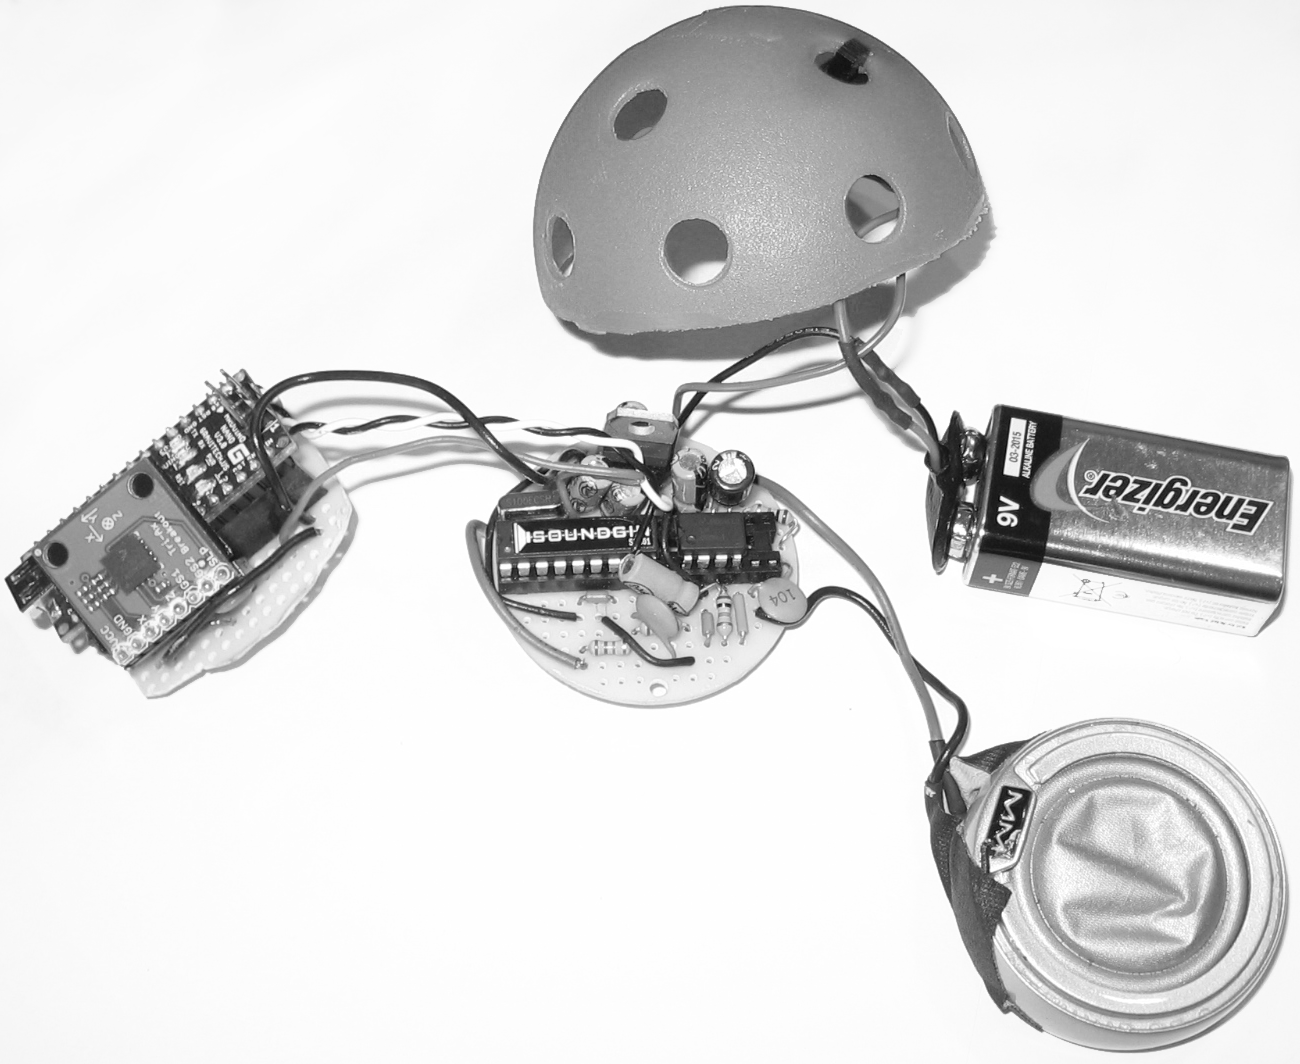
\includegraphics[scale=0.45]{beepinball_bw} %,width=1\textwidth
	\caption{The internals and half of the enclosure of a BeepinBall}
	\label{fig:beepinball}
\end{figure}

\begin{figure}[htbp]
	\centering
		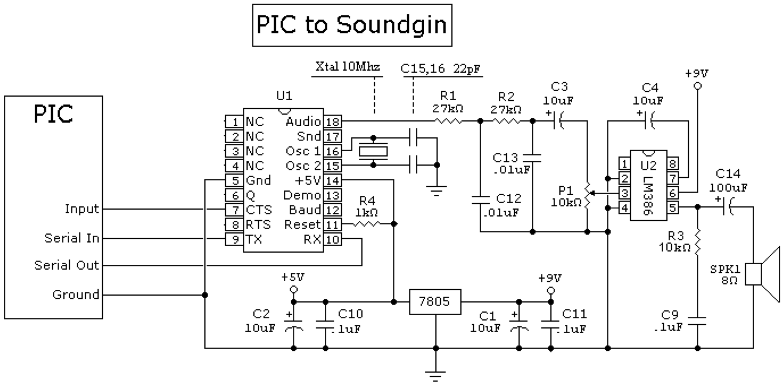
\includegraphics[scale=0.31]{soundballcircuit} %,width=1\textwidth
	\caption{The circuit diagram of the BeepinBall's controller$\Rightarrow$synthesizer$\Rightarrow$amplifier$\Rightarrow$speaker components}
	\label{fig:soundballcircuit}
\end{figure}

With this many electrical components jammed in next to one another, we 
inevitably had a number of issues arise from jostled connections or momentary
shorts during high-G moments such as when the ball is caught. These problems
were mostly alleviated by wrapping each circuit component tightly and 
thoroughly with gaffers tape. This served as both insulation from any other stray
leads and as shock-absorption and padding, minimizing the amount of movement
happening inside the ball. We also learned that 9-volt battery connectors are
generally unfit for being jostled and shaken, as they will lose contact
for brief moments with the battery leads. This caused the Arduino to
reset, halting sound output for several seconds. We had to tighten the snaps
on all of our connectors with pliers to stop the drop-outs from occurring.

\section{Firmware and Synthesis}

The behavior of the synthesizer is entirely determined by custom firmware 
loaded onto the Arduino's ATmega 328 microcontroller chip. This code, written
using functions from the Arduino C libraries, has several high-level modules 
which interact but are encapsulated from one another. 

First, the firmware measures the values from each of the accelerometer's three axes,
and then computes the instantaneous jerk (derivative of acceleration) and deviation 
from freefall (magnitude of the three-axis acceleration vector).\footnote{Because 
each axis of the accelerometer measures positive 
and negative deviation from a non-zero and possibly device-dependent baseline
value, the BeepinBall enters a 10-second calibration phase immediately after
starting up wherein the user must rotate the ball around its center as 
uniformly and completely as possible while the controller averages the 
values from each axis to find the baseline for that device.} 

Those values are then fed into prerequisite-checking functions for each state 
of a simple state machine, which compare the accelerometer values to various 
thresholds as well as only allowing transitions between certain states to enforce
basic sanity upon the system. The states in the machine are FREEFALL, CATCH, 
FORCE APPLIED, and AT REST. These correspond to the ball flying through the 
air, absorbing great force at the instant of impact, being moved by some 
force, or staying perfectly stationary. 

Finally, the state machine's current status is translated into commands 
for the synthesizer, typically based on what state the ball is in (what type 
of sound to make), how long it has been in that state (if the sound is 
time-varying), and what the current accelerometer values are (if the sound 
varies in correspondence with the ball's motion).

\section{Interaction and Sound Design}

Currently, the sounds that emanate from a BeepinBall are entirely based on the state
of the ball and how long it has been in that state. In the FORCE APPLIED state, 
a droning tone plays while the user moves or carries the ball. From that state, it is
possible to transition to either AT REST if the player stops moving or FREEFALL if the
ball is thrown. AT REST results in silence until the next state change, whereas FREEFALL
triggers a rapidly ascending scale of beeps. This ascending scale continues until the ball 
is caught, when it briefly enters the CATCH state and a high-pitched ``bonk'' sound 
is played to emphasize the impact. After that, the ball may transition back into FORCE APPLIED
or AT REST.

One unintentional form of play with BeepinBalls that emerged was that 
players will often experiment with applying a physical filter to the FORCE APPLIED drone 
tone by moving the ball with one hand and covering the front of the speaker with the other, 
and then moving the covering hand like a trumpet mute, causing a wah-wah-like effect. 

\section{Conclusions and Future Work}

Our current revision of the BeepinBalls is functional but unpolished. The sounds in the 
current firmware are only placeholders, and do not reflect the motion of the ball to the 
degree we would like. The final sound synthesis will be more closely tied to the actual 
values from the accelerometer instead of relying only on the current state. The circuit
design and enclosure also need to be made much more robust, removing all external tape,
eliminating the possibility of switching off the ball with an unfortunate catch, and
making the whole circuit and interconnections more shockproof and strong. Lastly, we
hope to refine the circuit design further, ideally even creating a printed circuit board
so that BeepinBalls can be produced in greater quantity and more efficiently. We also
plan to run extensive user experience testing to gauge response, determine usability 
tweaks and get a sense of how much fun playing with BeepinBalls actually is.

In conclusion, BeepinBalls are hand-held toy balls which contain miniature synthesizers
and can add a new sonic dimension to the universal human experience of playing with 
balls, particularly the act of juggling. We designed and created hardware and circuitry
that is extremely small and robust to ensure that natural play could occur, without concern of 
breakage. The sound design is aimed at rewarding exploratory play and allowing expressive 
physical manipulation of the balls to create a correspondingly expressive sonic output. 

In early testing, we have seen exactly this desired outcome bear out: people start to play 
with the balls, and quickly enter a feedback loop wherein their manipulations trigger sounds 
which lead them to build a mental model of the balls' behavior, which they then continue to 
flesh out by experimenting with further physical manipulations. This validates our theory that 
adding sonic output to playing with balls can indeed enrich even such a fundamental play experience, and was 
extremely satisfying to observe.

\end{document}
